%
%  Vincent Yannello
%
\documentclass[12pt,fullpage]{article}
\usepackage{fullpage}
\usepackage{amsmath}
\DeclareMathOperator{\erf}{erf}
\usepackage{psfrag}                                          % LaTeX graphics tool
\usepackage{pslatex}                                         % avoids the default cmr font
\usepackage{graphicx}                                        % graphics package 
\usepackage{epsfig}                                          % figures
\usepackage{hyperref}
\usepackage{color}

\begin{document}

\noindent
{\bf Minimax distribution} (from \color{blue}\url{http://www.math.wm.edu/~leemis/chart/UDR/UDR.html}\color{black})

\noindent
The shorthand $X \sim {\rm minimax}(\beta,\, \gamma)$ is used to indicate that the
random variable $X$ has the minimax distribution with positive shape parameters $\beta$ and $\gamma$.
A minimax random variable $X$ with parameters~$\beta$ and $\gamma$ has probability density function 
$$
f(x) = {\it \beta} \,\gamma \, {x} ^ {{\kern 0.08 em \beta} - 1} \left( 1 - {x} ^ {{\kern 0.08 em \beta}}
 \right) ^ {\kern -0.08 em \gamma - 1} \qquad \qquad 0< x < 1.
$$
The probability density function with three different parameter settings is illustrated below.
{\begin{figure}[h!]
\begin{center}
\psfrag{lab1}{$\alpha \kern -0.08 em = \kern -0.08 em  2,\, \beta \kern -0.08 em  = \kern -0.08 em  2$}
\psfrag{lab2}{$\alpha \kern -0.08 em  = \kern -0.08 em  1,\, \beta \kern -0.08 em  = \kern -0.08 em  3$}
\psfrag{lab3}{$\alpha \kern -0.08 em  = \kern -0.08 em  0.5,\, \beta \kern -0.08 em  = \kern -0.08 em  0.5$}
\psfrag{labx}{$x$}
\psfrag{labf}{$f(x)$}
\includegraphics[width=3.2in]{MinimaxPlot.ps}
\end{center}
\end{figure}}\\
The cumulative distribution on the support of $X$ is
$$
F(x) = P(X \leq x) = 1 - \left(1 - x ^ {\kern 0.08 em \beta} \right) ^ \gamma \qquad \qquad 0 < x < 1.
$$
The survivor functionx on the support of $X$ is
$$
S(x) = P(X \geq x) = \left(1 - x ^ {\kern 0.08 em \beta} \right) ^ \gamma \qquad \qquad 0 < x < 1.
$$
The hazard function on the support of $X$ is
$$
h(x) = \frac{f(x)}{S(x)} = {\frac {{\beta} \, \gamma \, {x} ^ {{\kern 0.08 em \beta} - 1}}{1 - {x} ^ {{\kern 0.08 em
 \beta}}}} \qquad \qquad 0 < x < 1.
$$
The inverse distribution function of $X$ is
$$
F ^ {-1}(u) = \left(1 - (1 - u) ^ {1 / \gamma} \right) ^ {\kern -0.08 em 1 / \beta} \qquad \qquad 0 < u < 1.
$$
The cumulative hazard, moment generating, and characteristic functions on 
the support of $X$ are mathematically intractable.\\
\\
\noindent
The population mean of $X$ is
$$
E[X] = \frac{\Gamma  \left( \gamma + 1 \right) \Gamma  \left( {({\beta} + 1)/{\beta}} \right)} {\Gamma  \left( ({\beta} \, \gamma + {\beta
} + 1)/{\beta} \right)} \qquad \qquad. 
$$

\vspace{0.1in}

%\noindent
%{\bf APPL verification:}
%The APPL statements
%\begin{verbatim}
%assume(beta > 0);
%assume(y > 0);
%X := [[x -> beta*y*x^(beta-1)*(1-x^(beta))^(y-1)],[0,1],["Continuous", "PDF"]];
%CDF(X);
%SF(X);
%HF(X);
%IDF(X);
%Mean(X);
%\end{verbatim}
%verify the cumulative distribution function, survivor function, hazard function, inverse function, and the population mean.

\end{document}
